

\begin{figure}[h]
    \centering
    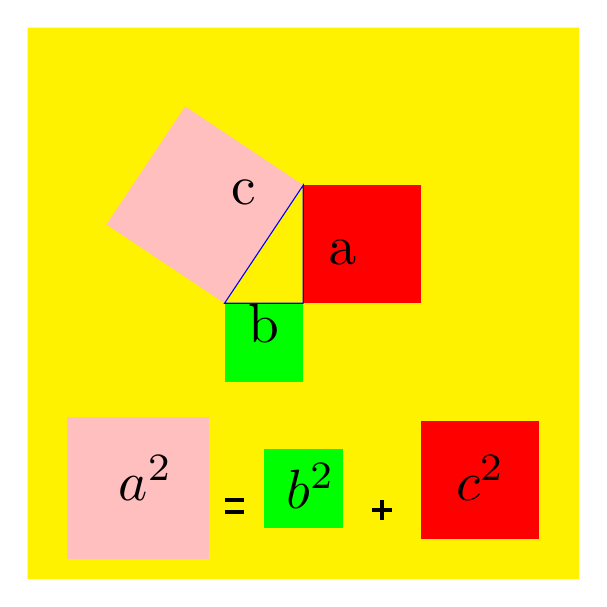
\begin{tikzpicture}[scale=0.5]
        %\draw [help lines] (-10,-10) grid (10,10);
        
        %\draw [red, fill=red, ultra thick] (4,4) circle [radius=.1];
        %\path [blue, fill=red, ultra thick] (-10,0) to [out=135, in=180] (0,5) to [out=0, in=45] (10,0) -- (-10,0);
        %\draw [red, domain=-4*pi:4*pi, line width=3pt, samples=50] plot (\x,{5*sin(\x r/2)});
        
        %\node [below right, scale=2] at (4,4) {A};
        
        
        %the main figure starts
        
        %\path [fill=yellow] (0,4) to [out=0, in=180] (10,1) -- (10,0) -- (0,0) -- (0,4);
        %\draw [blue, ultra thick] (-10,1) to [out=0, in=180] (0,4) to [out=0, in=180] (10,1);
        %\draw [thick, ->] (2,2) to [out=-135, in=180] (5,-5);
        
        %\draw [thick, <->] (-10,0) -- (10,0);
        %\draw [thick, <->, rounded corners] (0,10) -- (0,-10);
        
        %\node [below left, scale=2] at (10,0) {$x$};
       % \node [above, scale=2] at (0,10) {$f(x)$};
       % \node [right, scale=2] at (5,-5) {$A = \int_{x=0}^{\infty}f(x) dx$};
       \path [fill=yellow] (-7,-7) to [out=0, in=180] (7,-7) -- (7,7) -- (-7,7) -- (-7,-7);
       \path[fill=pink] (0,3) -- (-3,5) -- (-5,2) --(-2,0)--(0,3);
       \path[fill=red] (0,0)  rectangle(3,3);
       \path [fill=green] (0,0) rectangle(-2,-2);
       \draw[blue] (0,0)--(0,3)--(-2,0)--(0,0);
       %\draw (-3,0) to (0,4) rectangle(5,5);
       %\draw [blue] (2,0) --  (2,4) -- (-1,0) --(2,0); 
       %\path[fill=pink] (0,4)--(4,1)--(-4,1)--(-3,0);
        \path[fill=pink] (-6,-6.5) rectangle(-2.4,-2.9);
         \draw[ultra thick] (-2,-5)--(-1.5,-5);
       \draw[ultra thick] (-2,-5.3)--(-1.5,-5.3);
      \path[fill=green] (-1,-5.7) rectangle(1,-3.7);
      \draw[ultra thick] (2,-5)--(2,-5.5);
      \draw[ultra thick] (2.25,-5.25)--(1.75,-5.25);
       \path[fill=red] (3,-6) rectangle(6,-3);
       \node[above,scale=2] at (-1,-1.5) {b};
       \node[above,scale=2] at (1,.5) {a};
       \node[above,scale=2] at (-1.5,2) {c};
        \node [above, scale=2] at (-4,-5.5) {$a^2$};
        \node [above left, scale=2] at (1.3,-5.7) {$b^2$};
          \node [above, scale=2] at (4.5,-5.5) {$c^2$};

         \end{tikzpicture}
    \caption{Visual representation of the famous Pythagorean theorem.}
\end{figure}

\begin{figure}[h]
    \centering
    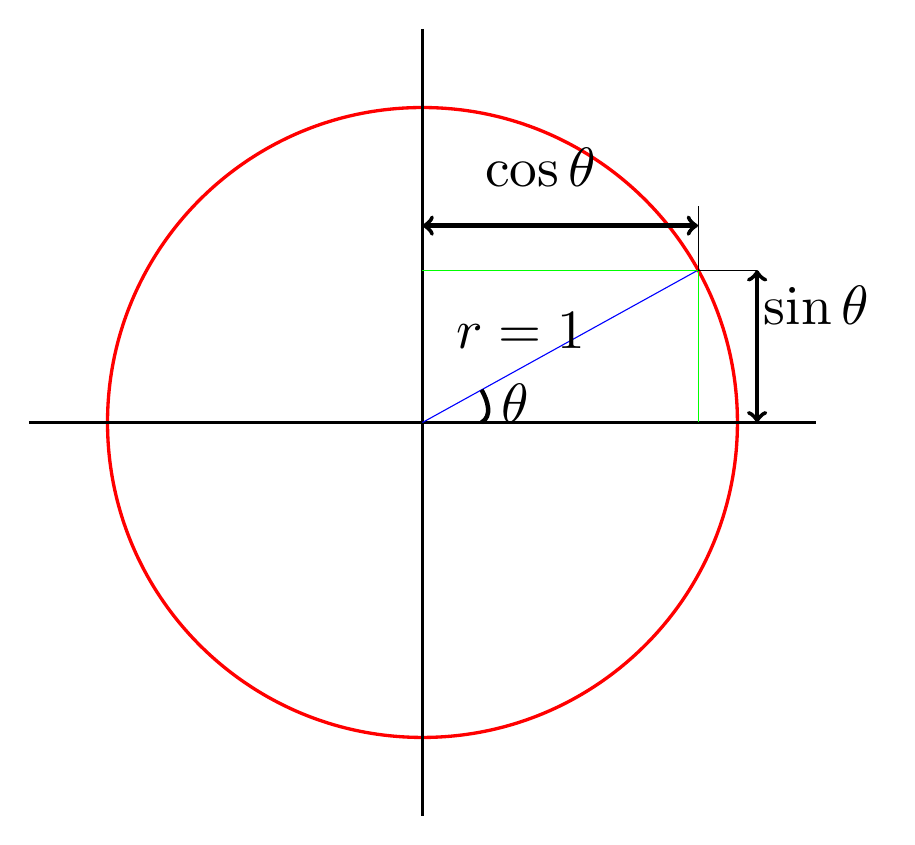
\begin{tikzpicture}[scale=0.5]
     \draw [red,very thick] (0,0) circle [radius=8];
    \draw [thick] (-10,0) -- (10,0);
    \draw [thick] (0,10) -- (0,-10);
    \draw[blue] (0,0)--(7,3.87);
    \draw[green] (7,0)--(7,3.87);
    \draw[green] (7,3.87)--(0,3.87);
    \draw[ultra thick,<->] (0,5)--(7,5);
    \draw[black] (7,3.87) to (7,5.5);
    \node[above,scale=2] at (3,5.5) {$\cos{\theta}$};
     \draw[ultra thick,<->] (8.5,0)--(8.5,3.87);
     \draw[ultra thick] (1.5,0)to [out=30,in=-60](1.5,.829);
    \draw[black] (7,3.87) to (8.5,3.87);
    \node[above,scale=2] at (10,2) {$\sin{\theta}$};
    \node[above,scale=2] at (2.5,1.382) {$r=1$};
    \node[right,scale=2] at (1.5,.5) {$\theta$};
    \end{tikzpicture}
    \caption{ Alternate representation of Pythagorean theorem.};
\end{figure}